\subsection{Akwizycja danych}
W projekcie założono wykorzystanie metod fotogrametrycznych do tworzenia trójwymiarowych modeli obszarów urbanistycznych. Za część projektu przyjęto z tego względu również pozyskanie własnych
zestawów danych fotograficznych (fotogramów), które spełniałyby wymogi techniczne, umożliwiające
późniejszą rekonstrukcję 3D. Wynikowe zbiory zdjęć powstały poprzez wykonanie dużej liczby ujęć, obejmujących wiele kątów i perspektyw oraz zapewniając odpowiednie nakładanie się obrazów dla poprawnego działania oprogramowania fotogrametrycznego.


Akwizycję zrealizowano na kampusie Politechniki Wrocławskiej, koncentrując się na budynkach C5,
C7 oraz Strefie Kultury Studenckiej (SKS)[\ref{fig:four-photos}] i pozyskując zdjęcia zarówno z lotów bezzałogowym statkiem powietrznym, jak i z poziomu gruntu. W jej wyniku przygotowano własne kompletne zbiory danych, które spełniły wymogi jakościowe i posłużyły do budowy testowych modeli.

\begin{figure}[h!]
    \centering
    \begin{minipage}{0.24\textwidth}
        \centering
        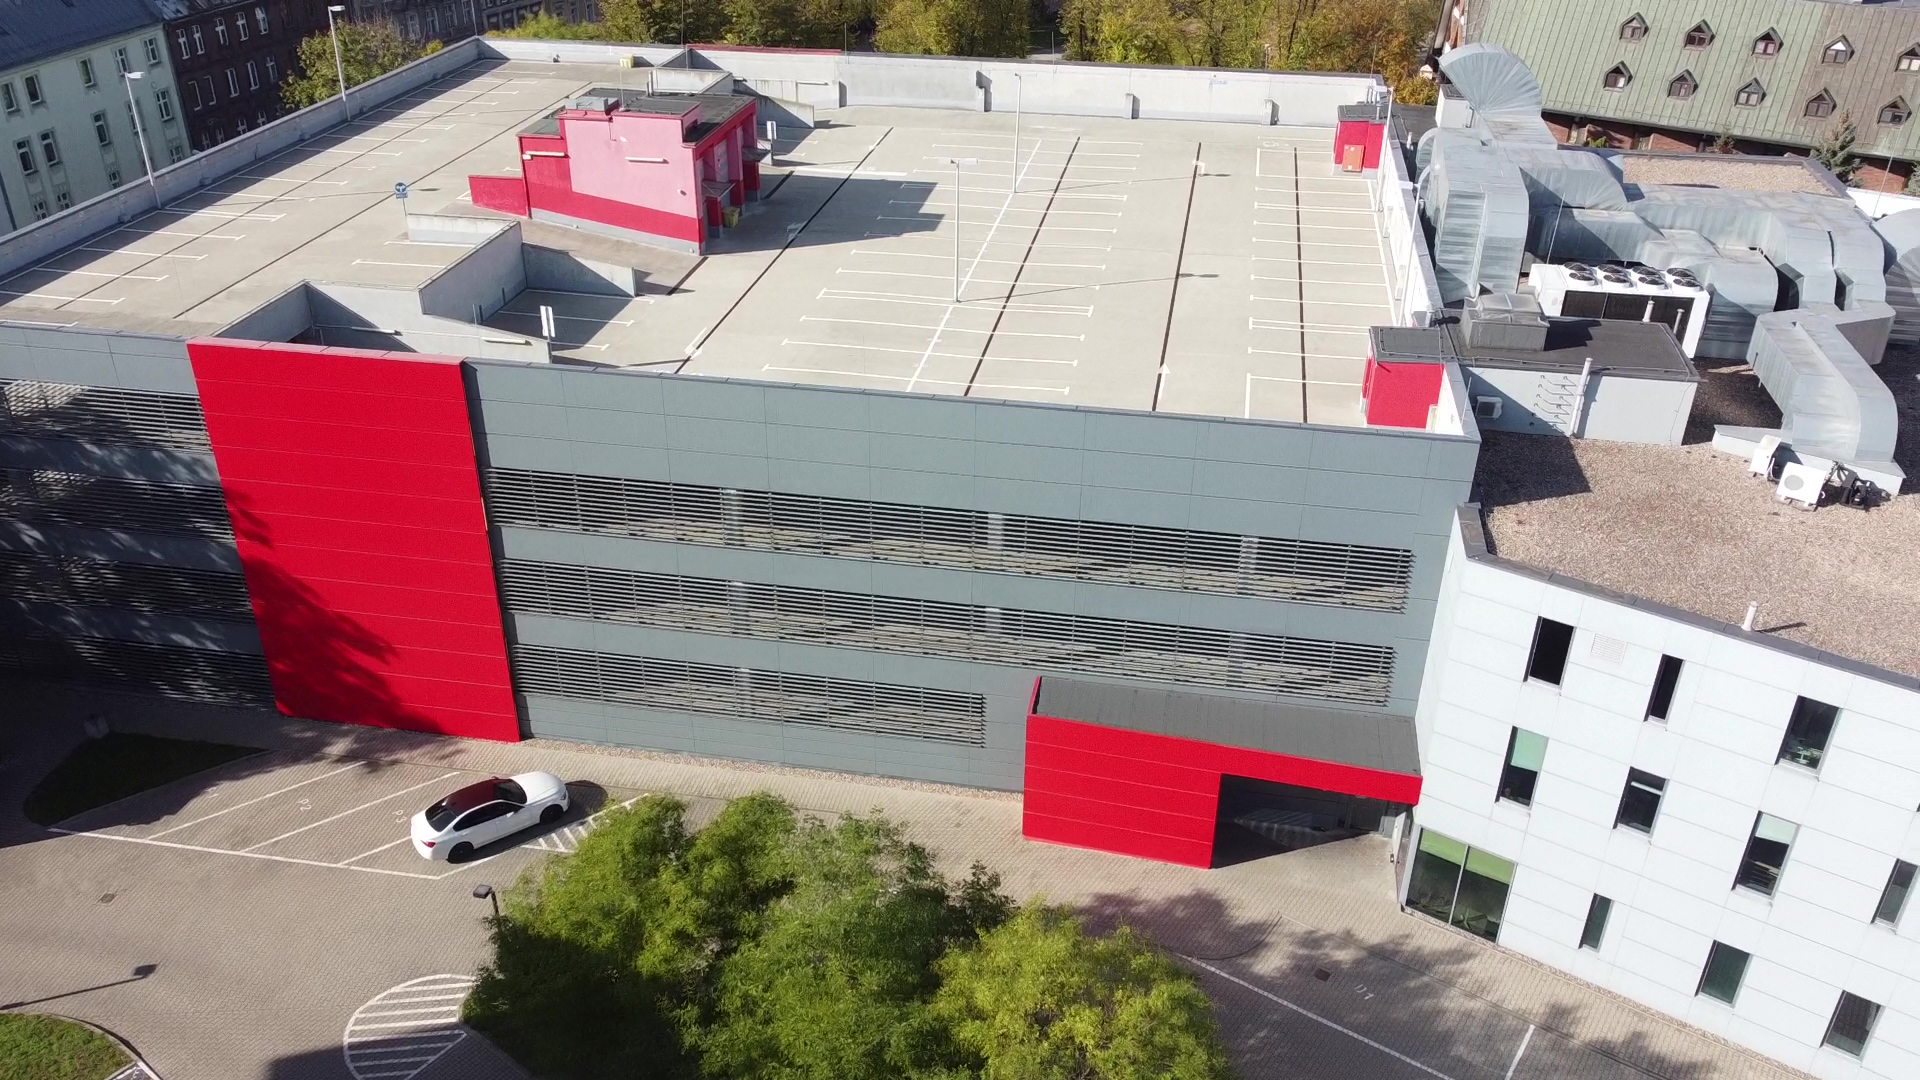
\includegraphics[width=\textwidth]{img/sks_dataset_1.jpg}
    \end{minipage}
    \hfill
    \begin{minipage}{0.24\textwidth}
        \centering
        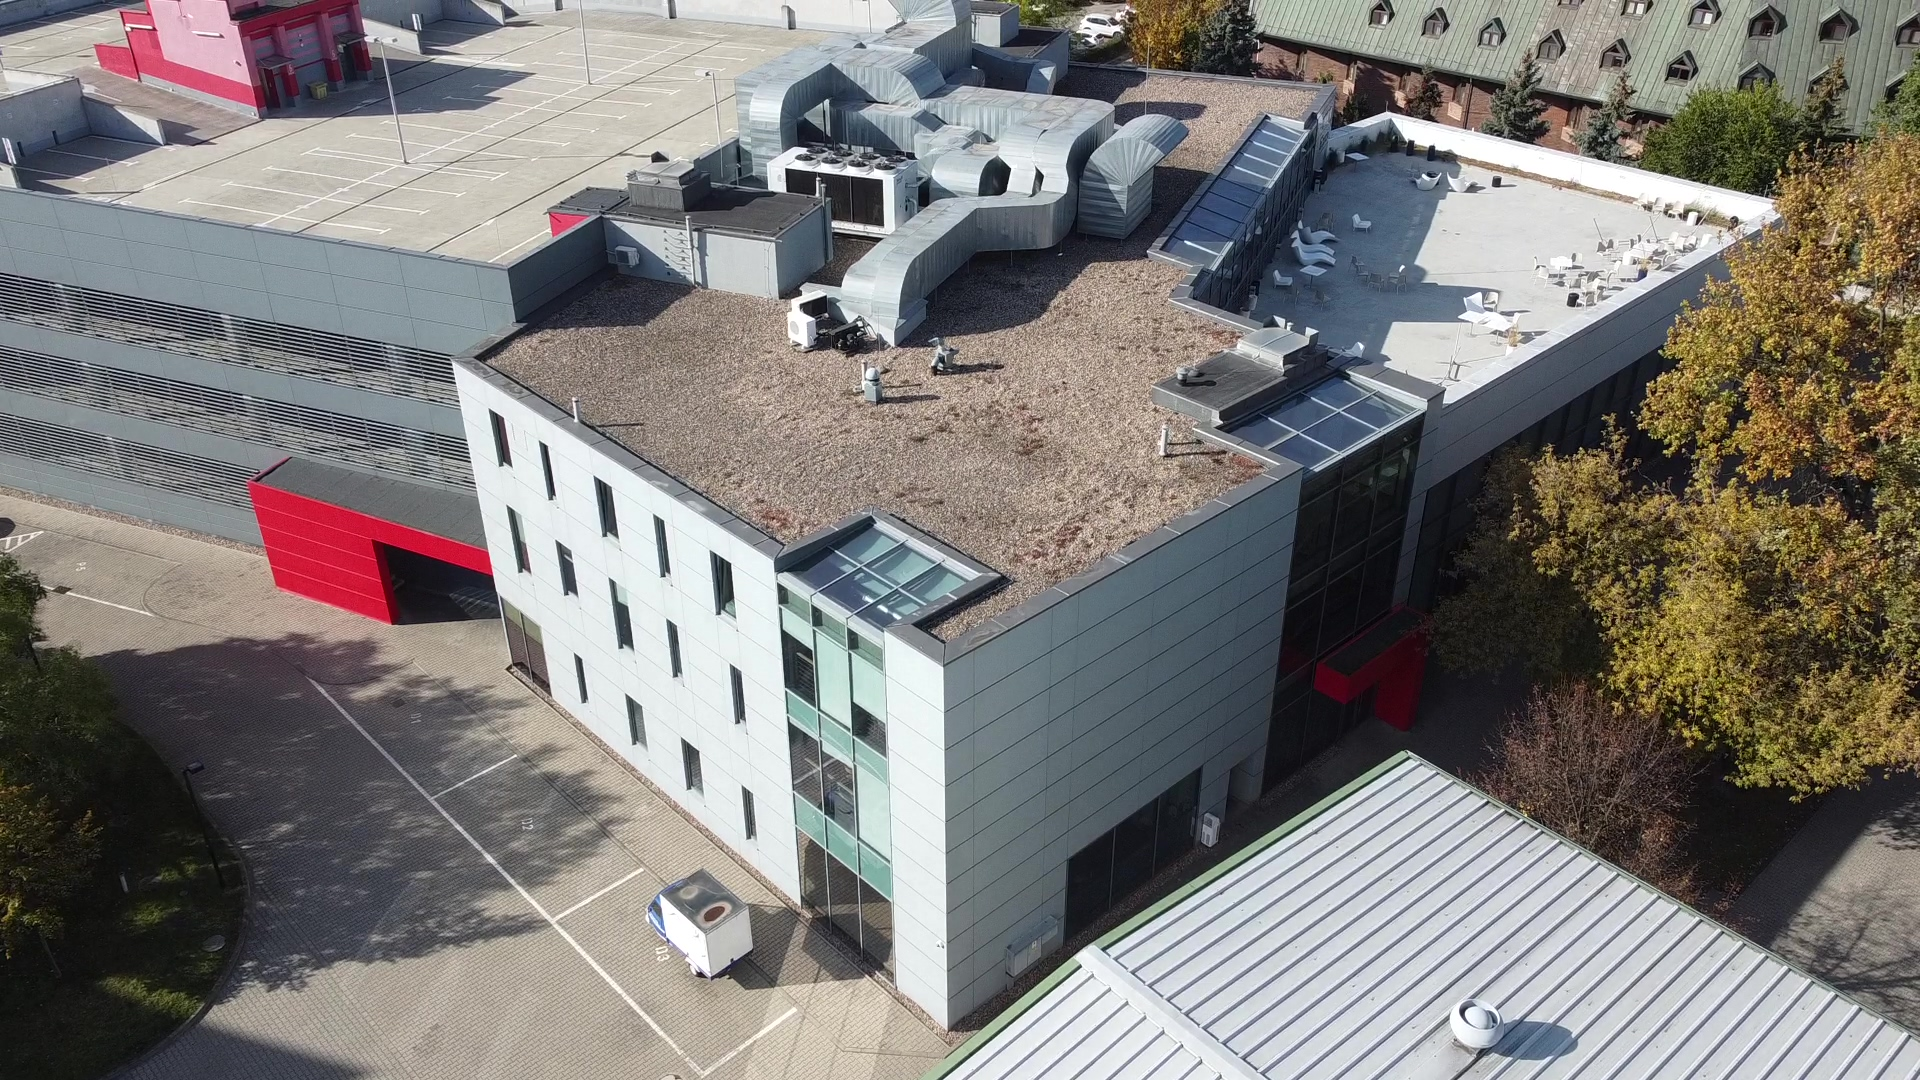
\includegraphics[width=\textwidth]{img/sks_dataset_2.jpg}
    \end{minipage}
    \hfill
    \begin{minipage}{0.24\textwidth}
        \centering
        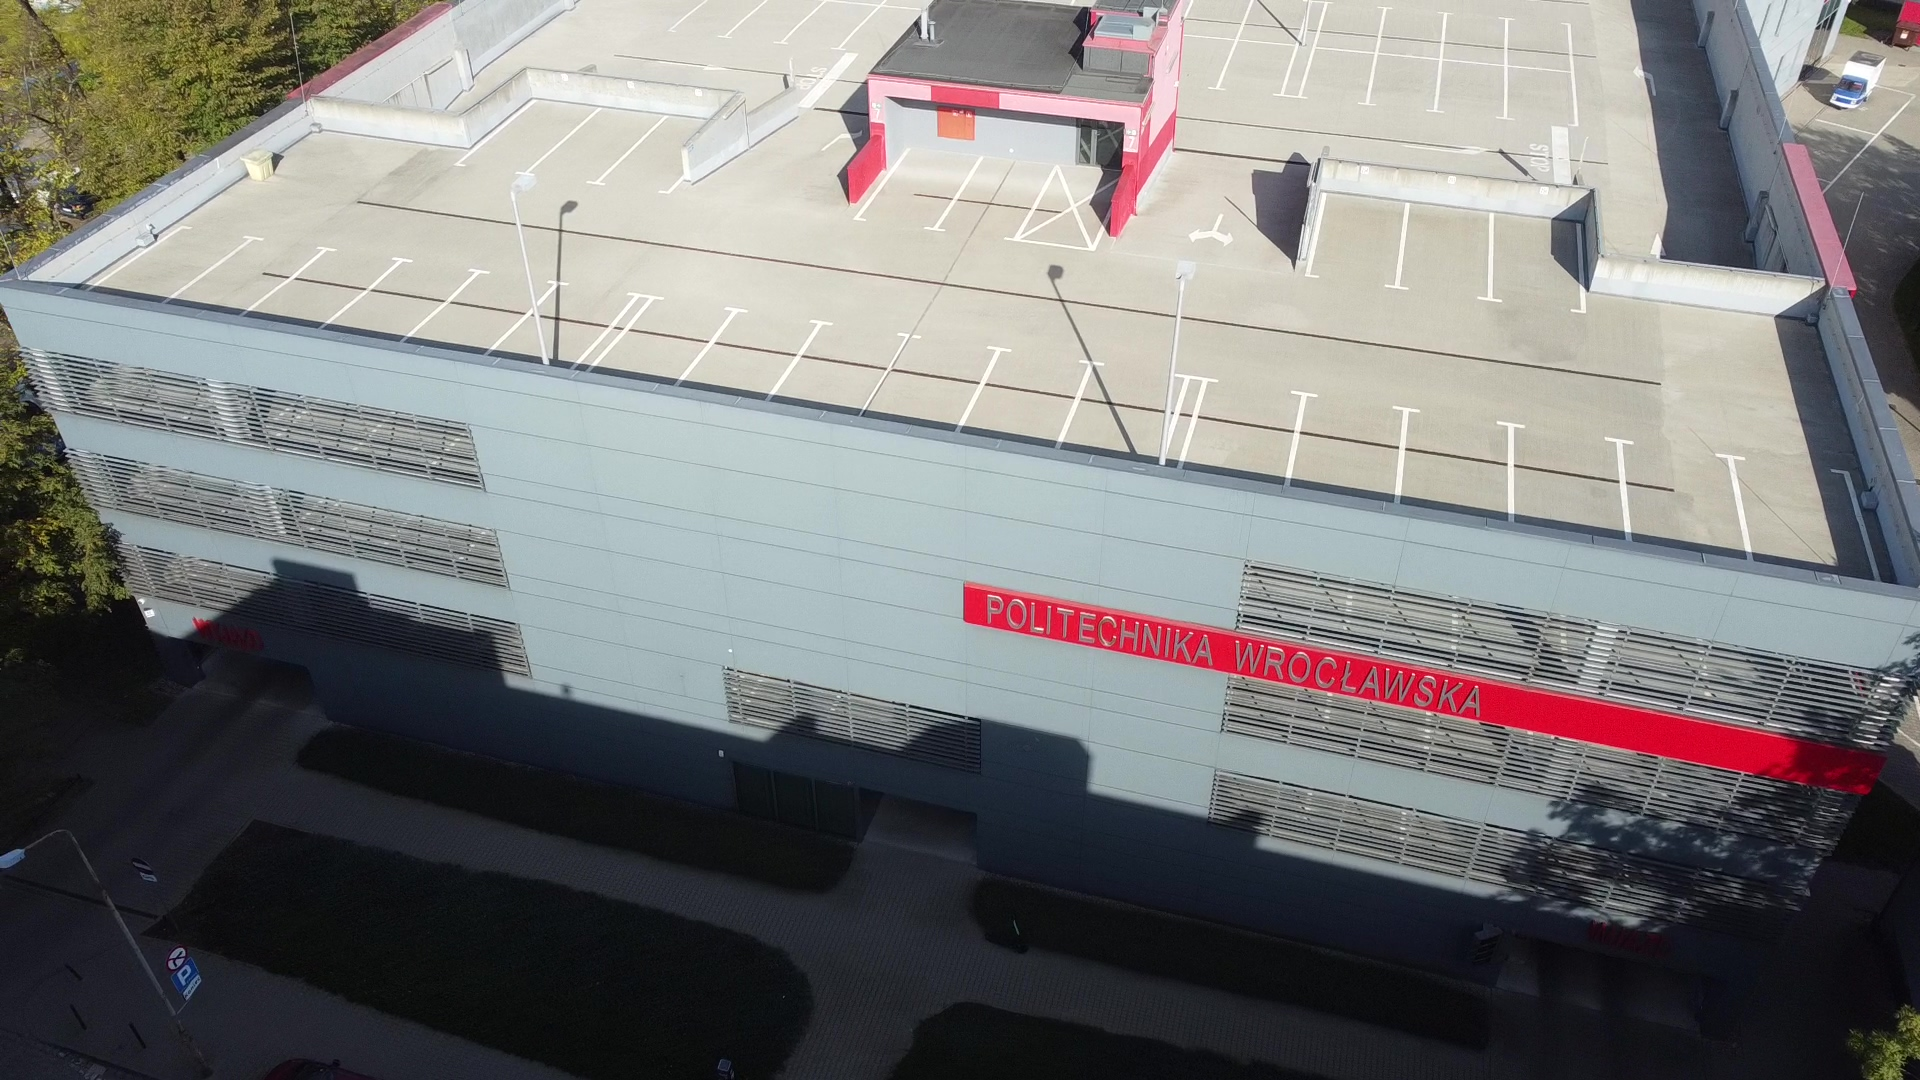
\includegraphics[width=\textwidth]{img/sks_dataset_3.jpg}
    \end{minipage}
    \hfill
    \begin{minipage}{0.24\textwidth}
        \centering
        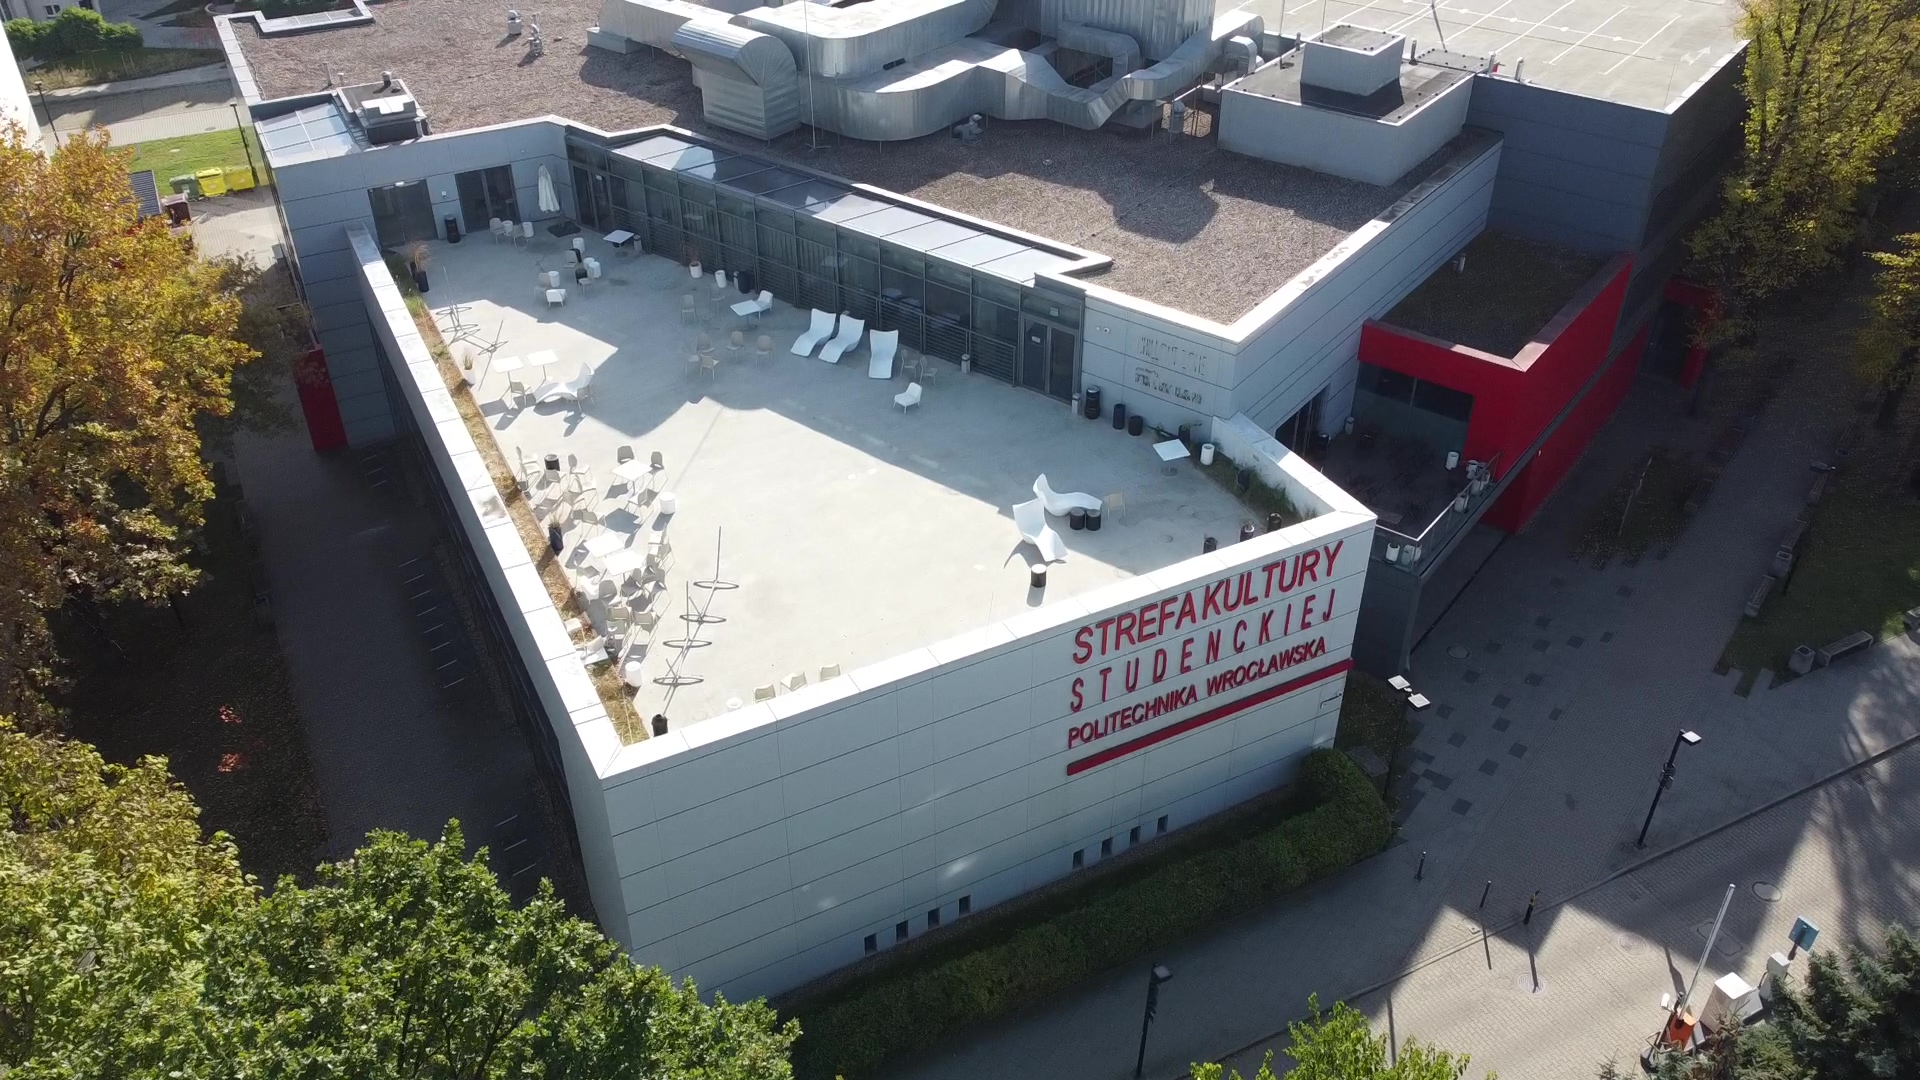
\includegraphics[width=\textwidth]{img/sks_dataset_4.jpg}
    \end{minipage}
    \caption{Przykładowe zdjęcia z akwizycji danych przedstawiające SKS}
    \label{fig:four-photos}
\end{figure}